\documentclass[a4paper, 12pt]{article}
\usepackage[utf8]{inputenc}
\usepackage[english,russian]{babel}
\usepackage[warn]{mathtext}
\usepackage{graphicx}
\usepackage{float}
\usepackage{multirow}
\restylefloat{table}
\usepackage{amsmath}
\usepackage{floatflt}
\usepackage[T2A]{fontenc}
\usepackage[left=20mm, top=20mm, right=20mm, bottom=20mm, footskip=10mm]{geometry}

\tolerance 1414
\hbadness 1414
\emergencystretch 1.5em
\hfuzz 0.3pt        % размер максимального переполнения без warning'a
\widowpenalty=10000 % запрещает одиночную строку абзаца в начале страницы
\vfuzz \hfuzz
\raggedbottom       % если на странице мало содержимого, добавить пустое место в конце, а не в середине страницы



\begin{document}

\begin{titlepage}
	\centering
	\vspace{5cm}
	{\scshape\LARGE московский физико-технический институт (национальный исследовательский университет) \par}
	\vspace{6cm}
	{\scshape\Large Лабораторная работа 4.4.1 \par}
	{\huge\bfseries Изучение дифракционной решетки с помощью гониометра \par}
	\vspace{1cm}
	\vfill
\begin{flushright}
	{\large Б03-102}\par
	\vspace{0.3cm}
	{\LARGE Куланов Александр}
\end{flushright}
	

	\vfill


	Долгопрудный, 2023 г.
\end{titlepage}

\begin{itemize}
	\item \textbf{Цель работы:} Знакомство с работой гониометра и определение спектральных характеристик амплитудной или фазовой решетки (эшелета)
    \item \textbf{В работе используются:} ртутная лампа, гониометр, амплитудная и фазовая дифракционные решетки, плоскопараллельная стеклянная пластинка, призменный отражатель, щель с микрометричсеким винтом
\end{itemize}

\section{Теоретические сведения}
Дифракционная решётка представляет собой стеклянную или металлическую пластиику, на которую с помошьо делительной машины через строго одинаковые интервалы нанесены параллельные штрихи. В учебных лабораториях обычно применяются отнечатки таких гравированных решёток - реплики, изготозленные из специальной пластмассы.
Основными параметрами дифракциониой решётки являются её период $d$ (постоянная решётки) и число штрихов $N$.

Обычно дифракционная решётка освещается плоской волной (рис. 1). а плоскость наблюдения практически находится в бесконечности (условия дифракции Фраунгофера). В этом случае направление, в котором производится наблодение, определяется углом $\varphi$ между нормалью к решётке и направлением лучей.

\begin{figure}[H]
    \centering
    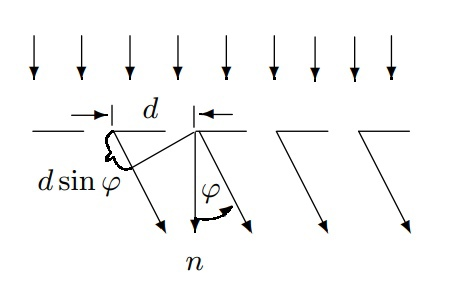
\includegraphics[width=0.5\textwidth]{ris2}
    \caption{Дифракция}
    \label{fig:ris1}
\end{figure}

В соответствии с принцином Гюйгенса-Френеля распределение интенсинности в дифракционной картине определяется суперпозицией волн, приходящих в точку наблодения от различных щелей решётки. При этом амплитуды всех интерферирующих волн при заданном угле $\varphi$ практически одинаковы, а фазы составляют арифметическую прогрессию.

Пусть падающая на решётку волна распространяется пернендикулярно её поверхности. Интенсивность дифрагированного света максимальна для углов $\varphi_m$, для которых волны, приходящие в точку наблодения от всех шелей решётки, оказываются в фазе.

Как следует из рис. \ref{fig:ris1}, для этих направлений справедииво соотношение
\begin{equation}
	d \sin \varphi_m=m \lambda \quad(m \quad \text { целое число). }
\end{equation}
Точная теория решётки учитывает как интерференцию волн, нриходящих от разных щелей, так и дифракцию на каждой щели. Как показывает простой расчёт, интенсивность I света, распространяющегося
под углом $\varphi$ к нормали, определяется формулой
\begin{equation}
I=I_1(\varphi) \frac{\sin ^2[N(k d \sin \varphi) / 2]}{\sin ^2[(k d \sin \varphi) / 2]},
\end{equation}
где $k=2 \pi / \lambda$ - волновое чисто, а множитель $I_1(\varphi)$ описывает дифракцию волн, испускаемых одним периодом решётки (диаграмма направленности одного периода).
Анализ выражения (2) показывает, что при большом числе щелей свет, прошедший через решётку, распространяется по ряду резко ограниченных направлений, определяемых соотношением (1). Зависимость интенсивности света от угла наблюдения представлена на puс. 2.

Как следует из (1), углы, при которых наблюдаются световые максимумы, зависят от длины волны $\lambda$. Дифракционная решетка, таким образом, предсталвяет собой спектральный прибор. Если на дифракционную решётку падает свет сложного спектрального состава, то после решётки образуется спектр, причём фиолетовые лучи отклоняются решёткой меньше, чем красные. 
Входящая в (1) величина $m$ носит название порядка спектра. При $m=0$ максимумы интенсивности для всех длин волн располагаются при $\varphi=0$ и накладываются друг на друга. При освешении белым светом нулевой максимум, в отличие от всех прочих, оказывается поэтому неокрашенным. Спектры первого, второго и т. д. порядков располагаются симметрично по обе стороны от нулевого.

\begin{figure}[H]
    \centering
    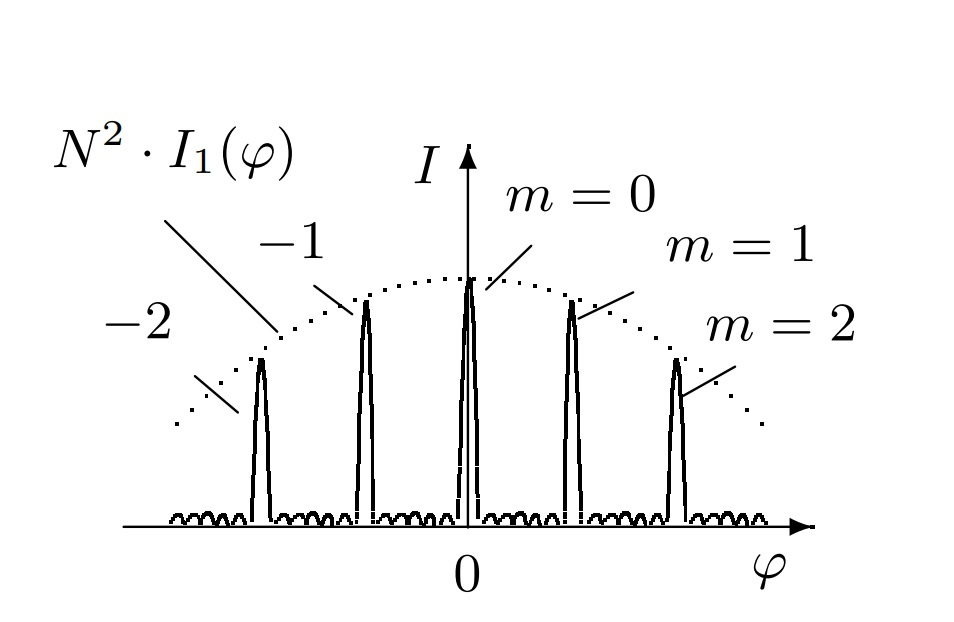
\includegraphics[width=0.5\textwidth]{ris3}
    \caption{Распределение интенсивностей}
    \label{fig:ris2}
\end{figure}

\subsection*{Угловая дисперсия.} 
Дисперсия $D$ характеризует угловое расстояние между близкими спектральными линиями:
\begin{equation}
D=\frac{d \varphi}{d \lambda} .
\end{equation}
Дифференцируя обе части (1), получим
\begin{equation}
d \cos \varphi d \varphi=m \cdot d \lambda \text {. }
\end{equation}
Следовательно,
\begin{equation}
D=\frac{d \varphi}{d \lambda}=\frac{m}{d \cos \varphi}=\frac{m}{\sqrt{d^2-m^2 \lambda^2}}
\end{equation}

Дисперсия возрастает с увеличением порядка спектра. На опыте дисперсию решётки отределяюот путём измерения углового расстояния $\Delta \varphi$ между двумя близкими спектральными линиями с известной разностью длин волн $\Delta \lambda$ (например, между жёлтыми линиями ртути).
\subsection*{Разрешающая способность дифракционной решётки.}

\begin{figure}[H]
    \centering
    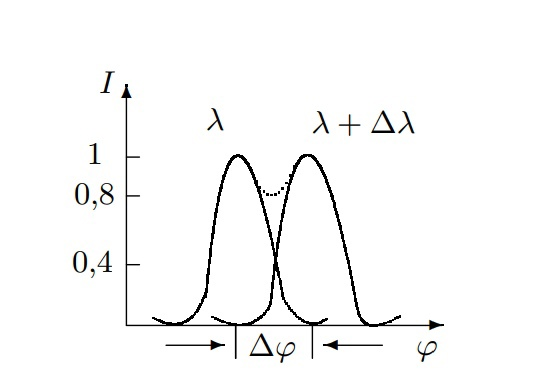
\includegraphics[width=0.5\textwidth]{ris4}
    \caption{К определению разрешающей способности дифракционной решетки}
    \label{fig:ris3}
\end{figure}

Возможность разрешения двух близких спектральньх линий зависит от их ширины и от расстояния между ними.
Пусть в спектре $m$-го порядка наблюдаются две близкие спектральные линии с длинами волн $\lambda$ и $(\lambda+\Delta \lambda)$. Угловое расстояние $\Delta \varphi$ между этими линиями, согласно (4), равно
\begin{equation}
	\Delta \varphi=\frac{m \Delta \lambda}{d \cos \varphi} \text {. }
\end{equation}
Согласно критерию разрешения Релея линии становятся неразличимыми, когда расстолние между ними меньше, чем расстояние от максимума одной линии до её первого минимума (рис. 3). Как следует из (2), при переходе из главного максимума $(\varphi=0)$ в минимум величина $N(k d \sin \varphi) / 2$ изменяется на $\pi$, так что
\begin{equation}
	\frac{N k d}{2}[\sin (\varphi+\delta \varphi)-\sin \varphi]=\pi \text {. }
\end{equation}
где $\delta \varphi$ - угловая полуширина главного максимума. Принимая во внимание малость $\delta \varphi$, получим из (7)
\begin{equation}
\delta \varphi=\frac{\lambda}{N d \cos \varphi} .
\end{equation}
Отметим, что угловая полуширина максимума обратно пропорциональна видимому размеру решётки $-N d \cos \varphi$.

По определению разрешающая способность спектрального прибора $R=\lambda / \delta \lambda$ - это отношение длины волны к разности длин волн двух линий, разрешаемых по критерияо Релея. Приравнивая $\delta \varphi$ и $\Delta \varphi$ для случая предельного разрешения, найдём для дифракционной решётки
\begin{equation}
R=\frac{\lambda}{\delta \lambda}=m \cdot N \text {. }
\end{equation}

Спектральный интервал $\delta \lambda$, входящий в соотношение (9), характеризует минимальное расстояние между двумя спектральными линиями, которые ещё могут быть разрешены при помощи данной дифракционной решётки.

\subsection*{Дисперсионная область.}
При достаточно широком спектральном интервале падающего света спектры разных порядков могут накладываться друг на друга. Предельная ширина спектрального интервала $\Delta \lambda$, при которой спектры соседних порядков ( $m$ и $m+1)$ перекрываются только своими границами, называется дисперсионной областъю $G$. При этом
\begin{equation}
d \sin \varphi=m(\lambda+\Delta \lambda)=(m+1) \lambda,
\end{equation}
и дисперсионная область
\begin{equation}
	G=\Delta \lambda=\frac{\lambda}{m}
\end{equation}


\section{Экспериментальная установка}
\begin{figure}[H]
    \centering
    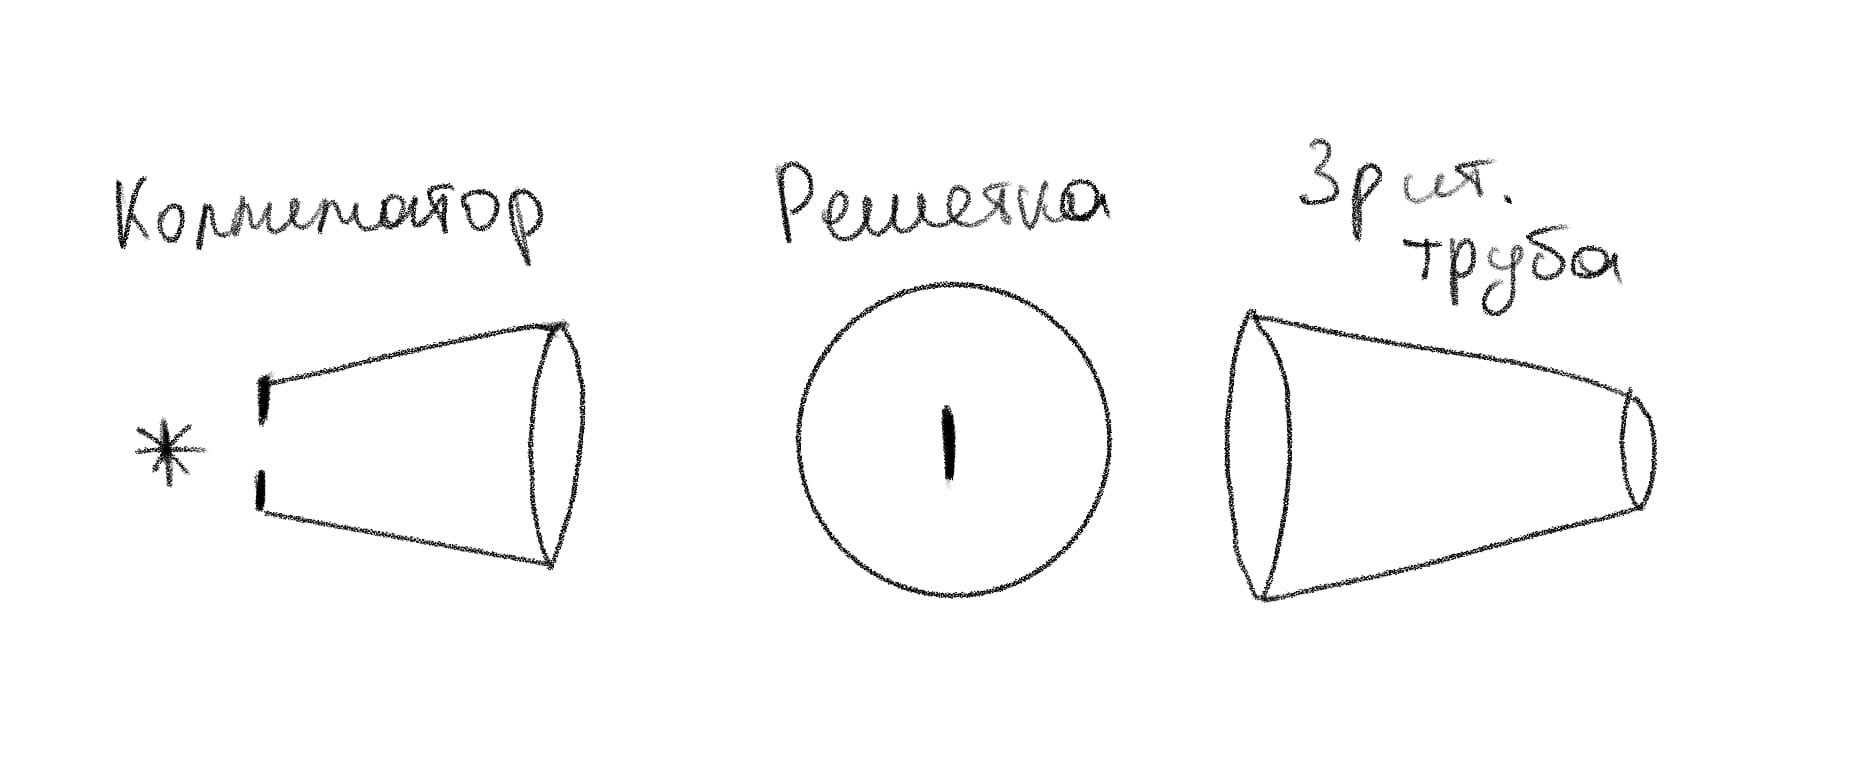
\includegraphics[width=1\textwidth]{ris1}
    \caption{Схема установки (сверху)}
    \label{fig:set}
\end{figure}

При работе с дифракционной решеткой основной задачей является точное измерение углов, при которых наблюдаются главные максимумы для различных длин волн. В нашей работе для измерения углов используется гониометр Г5, с устройством которого можно ознакомиться в описании работы 5.4. Принципиальная схема экспериментальной установки приведена на рис. 4.

\textbf{Измерение длин волн спектральных линий.} Дифракционная решётка с известным периодом может быть использована для измерения длин волн, например, в спектре ртути.
Как следует из (1), измерения длины волны сводятся к определению $\varphi_m$ - угла отклонения лучей от первоначального направления.
Проведя измерения дифракционных углов для спектра с известными длинами волн, можно рассчитать период решётки.
\textbf{Определение угловой дисперсии.} Для определения угловой дисперсии дифракционной решётки (см. формулу (3)) нужно измерить угловое расстояние $\Delta \varphi$ между двумя близкими спектральными линиями с длинами волн $\lambda_1$ и $\lambda_2$ и провести вычисления по формуле $D=\Delta \varphi /\left(\lambda_1-\lambda_2\right)$. \textbf{Оценка разрешающей способности решётки.} Непосредственное экспериментальное определение разрешающей способности дифракционной
решётки требует специальных источников света, в спектре которых имеются близкие спектральные линии, находящиеся на пределе разрешения. Обозначим через $\delta \lambda$ разность их длин волн. Разрешающая сила определяется отношением $\lambda / \delta \lambda$. При сравнении результатов с теоретической величиной разрешающей силы $(R=m N)$ необходимо принимать во внимание два обстоятельства.
1. Формула (9) была получена в предположении, что ширина спектральной линии обусловлена только дифракцией. Нетрудно сообразить, что дифракция определяет ширину спектральной линии лишь в том случае, если ширина щели $s$ коллиматора удовлетворяет соотношению
\begin{equation}
	\frac{s}{f} \ll \delta \varphi,
\end{equation}
где $f$ - фокусное расстояние объектива коллиматора, а $\delta \varphi$ - угловая полуширина дифракционного максимума. С помошью (8) для малых дифракционных углов найдём
\begin{equation}
	s \ll \frac{\lambda}{d N} f .
\end{equation}
При экспериментальной оценке разрешающей способности ширину щели коллиматора нужно выбирать достаточно малой. Полезно производить измерения при разных размерах щели, постепенно её уменьшая. Видимая ширина линии должна при этом сначала уменышаться вместе с шириной щели, а затем оставаться постоянной.
2. Иногда из-за плохого качества решёток получить чёткие спектральные линии удаётся только с помощью диафрагмы, установленной на коллиматорном объективе. Диафрагма позволяет выбрать достаточно однородный участок решётки, но при этом уменышает число освещённых штрихов решётки. В теоретической формуле $R=m N$ под $N$ нужно теперь понимать число одновременно работающих щелей, равное отношению ширины диафрагмы к периоду решётки. Однако даже при узких диафрагмах в экспериментах с решётками плохого качества нельзя быть
уверенным, что ширина наблюдаемых спектральных линий определяется только дифракцией (а не аберрациями).

Описанный метод позволяет измерить так называемую аппаратную или прибориую разрешаюпцую силу в реальных условиях опыта (т.е. при данных решётках, заданных размерах входной щели коллиматора, данном увеличении зрительной трубы и т.д.). Сравнение полученного результата с теоретическим (предельным) значением разрешающей силы позволяет оценить качество спектральной установки.
\section{Обработка результатов}
В ходе обработки выяснилось, что фиолетовый и два красных спектра были зафиксированы ошибочно. Отбросим их из данных.
Для +-1 порядка посмотрим на углы дифракции:

\begin{table}[H]
	\centering
	\begin{tabular}{|cccc|}
	\hline
	\multicolumn{4}{|c|}{\textbf{Ноль шкалы 180 14'43''}}                                                                                                                       \\ \hline
	\multicolumn{1}{|c|}{}                 & \multicolumn{1}{c|}{\textbf{$\lambda$, нм}} & \multicolumn{1}{c|}{\textbf{Угол, град. мин. сек.}} & \textbf{Угол, град. мин. сек.} \\ \hline
	\multicolumn{1}{|c|}{\textbf{Синий}}   & \multicolumn{1}{c|}{404,7}                  & \multicolumn{1}{c|}{192 01 11}                      & 168 10 17                      \\ \hline
	\multicolumn{1}{|c|}{\textbf{Голубой}} & \multicolumn{1}{c|}{491,6}                  & \multicolumn{1}{c|}{194 32 54}                      & 165 49 10                      \\ \hline
	\multicolumn{1}{|c|}{\textbf{Зелёный}} & \multicolumn{1}{c|}{546,1}                  & \multicolumn{1}{c|}{196 01 37}                      & 164 19 34                      \\ \hline
	\multicolumn{1}{|c|}{\textbf{Желтый}}  & \multicolumn{1}{c|}{577}                    & \multicolumn{1}{c|}{196 56 40}                      & 163 23 46                      \\ \hline
	\multicolumn{1}{|c|}{\textbf{Желтый}}  & \multicolumn{1}{c|}{579,1}                  & \multicolumn{1}{c|}{197 00 18}                      & 163 20 06                      \\ \hline
	\end{tabular}
	\caption{Данные об углах дифракции}
	\label{tab:data_1}
\end{table}

Вычтем из полученных углов ноль шкалы, переведем градусы в радианы, посчитаем синусы и занесем всё в таблицу:

\begin{table}[H]
	\centering
	\begin{tabular}{|c|c|c|c|}
	\hline
					 & \textbf{$\lambda$, нм} & \textbf{$\sin \varphi_1$} & \textbf{$\sin \varphi_{-1}$} \\ \hline
	\textbf{Синий}   & 404,7                  & 0,204                      & -0,209                        \\ \hline
	\textbf{Голубой} & 491,6                  & 0,247                      & -0,249                        \\ \hline
	\textbf{Зелёный} & 546,1                  & 0,272                      & -0,274                        \\ \hline
	\textbf{Желтый}  & 577                    & 0,287                      & -0,290                        \\ \hline
	\textbf{Желтый}  & 579,1                  & 0,288                      & -0,291                        \\ \hline
	\end{tabular}
	\caption{Синусы углов}
	\label{tab:data_2}
\end{table}

Построим графики зависимости $\sin \varphi_{\pm 1} = \pm \frac{1}{d} \lambda$. Угол наклона даст обратное значение для периода решетки:

\begin{figure}[H]
    \centering
    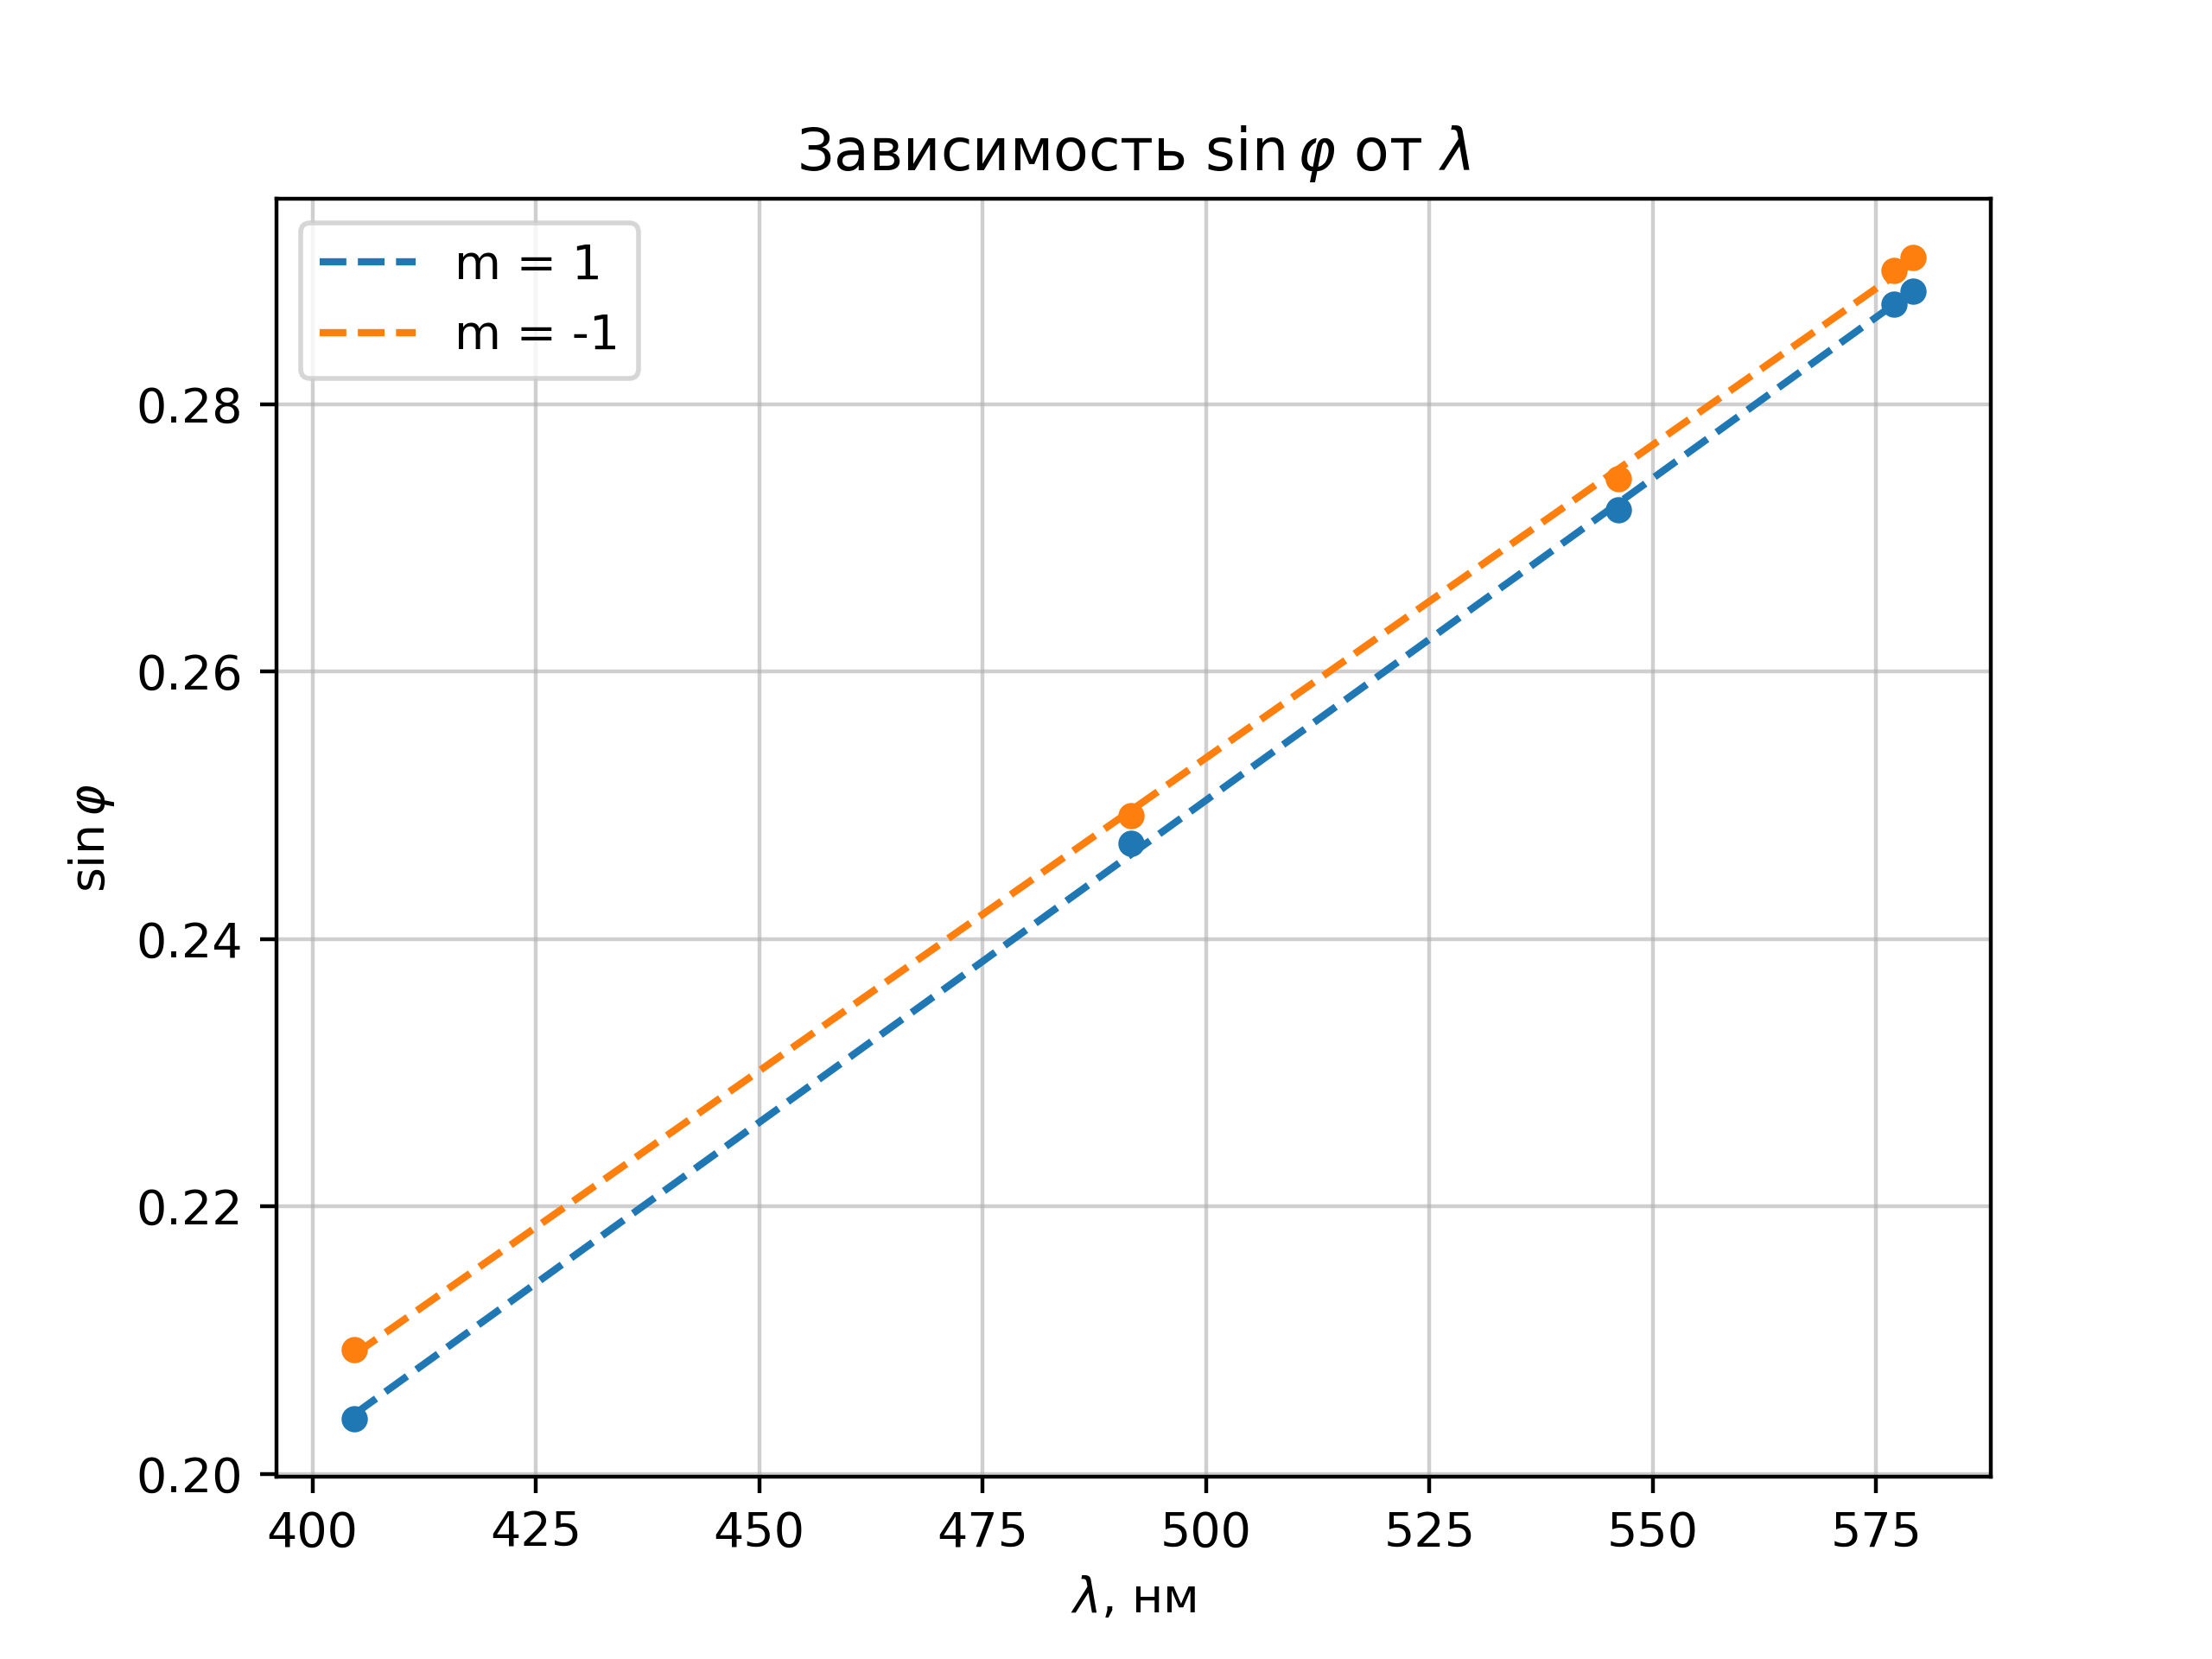
\includegraphics[width=1\textwidth]{plot1.png}
    \caption{Графики для синусов углов дифракции}
    \label{fig:plot1}
\end{figure}

Итого, проведя все расчеты, имеем

\begin{equation*}
	\boldmath{d = (2,1 \pm 0,2) \text{ мкм}} 
\end{equation*}
\begin{equation*}
	\boldmath{d_{\text{теор.}} = 2 \text{ мкм}}
\end{equation*}

Для расчёта угловой дисперсии приведем данные для желтых пар разных порядков:

\begin{table}[H]
	\centering
	\begin{tabular}{|cccc|}
	\hline
	\multicolumn{4}{|c|}{\textbf{Пары желтых   спектров}}                                                               \\ \hline
	\multicolumn{1}{|c|}{m}  & \multicolumn{1}{c|}{Угол}      & \multicolumn{1}{c|}{Угол, сек} & Угол, $\Delta$ сек     \\ \hline
	\multicolumn{1}{|c|}{1}  & \multicolumn{1}{c|}{196 56 24} & \multicolumn{1}{c|}{708984}    & \multirow{2}{*}{231}   \\ \cline{1-3}
	\multicolumn{1}{|c|}{1}  & \multicolumn{1}{c|}{197 00 15} & \multicolumn{1}{c|}{709215}    &                        \\ \hline
	\multicolumn{1}{|c|}{2}  & \multicolumn{1}{c|}{215 11 51} & \multicolumn{1}{c|}{774711}    & \multirow{2}{*}{495}   \\ \cline{1-3}
	\multicolumn{1}{|c|}{2}  & \multicolumn{1}{c|}{215 20 06} & \multicolumn{1}{c|}{775206}    &                        \\ \hline
	\multicolumn{1}{|c|}{3}  & \multicolumn{1}{c|}{239 00 06} & \multicolumn{1}{c|}{860406}    & \multirow{2}{*}{1177}  \\ \cline{1-3}
	\multicolumn{1}{|c|}{3}  & \multicolumn{1}{c|}{239 19 43} & \multicolumn{1}{c|}{861583}    &                        \\ \hline
	\multicolumn{1}{|c|}{-1} & \multicolumn{1}{c|}{163 23 46} & \multicolumn{1}{c|}{588226}    & \multirow{2}{*}{-220}  \\ \cline{1-3}
	\multicolumn{1}{|c|}{-1} & \multicolumn{1}{c|}{163 20 06} & \multicolumn{1}{c|}{588006}    &                        \\ \hline
	\multicolumn{1}{|c|}{-2} & \multicolumn{1}{c|}{144 42 41} & \multicolumn{1}{c|}{520961}    & \multirow{2}{*}{-523}  \\ \cline{1-3}
	\multicolumn{1}{|c|}{-2} & \multicolumn{1}{c|}{144 33 58} & \multicolumn{1}{c|}{520438}    &                        \\ \hline
	\multicolumn{1}{|c|}{-3} & \multicolumn{1}{c|}{118 57 40} & \multicolumn{1}{c|}{428260}    & \multirow{2}{*}{-1429} \\ \cline{1-3}
	\multicolumn{1}{|c|}{-3} & \multicolumn{1}{c|}{118 33 51} & \multicolumn{1}{c|}{426831}    &                        \\ \hline
	\end{tabular}
	\caption{Данные для желтых спектров}
	\label{tab:data_3}
\end{table}

Зная, что $\Delta\lambda$ для желтой пары 2,1 нм или 21 \r{A}, посчитаем $d\varphi/d\lambda$ и построим графики:

\begin{table}[H]
	\centering
	\begin{tabular}{|c|c|}
	\hline
	\textbf{m} & \textbf{D, сек/Ангстрем} \\ \hline
	1          & 11,00                    \\ \hline
	2          & 23,57                    \\ \hline
	3          & 56,05                    \\ \hline
	-1         & -10,48                   \\ \hline
	-2         & -24,90                   \\ \hline
	-3         & -68,05                   \\ \hline
	\end{tabular}
	\caption{Угловые дисперсии}
	\label{tab:data_4}
\end{table}

\begin{figure}[H]
    \centering
    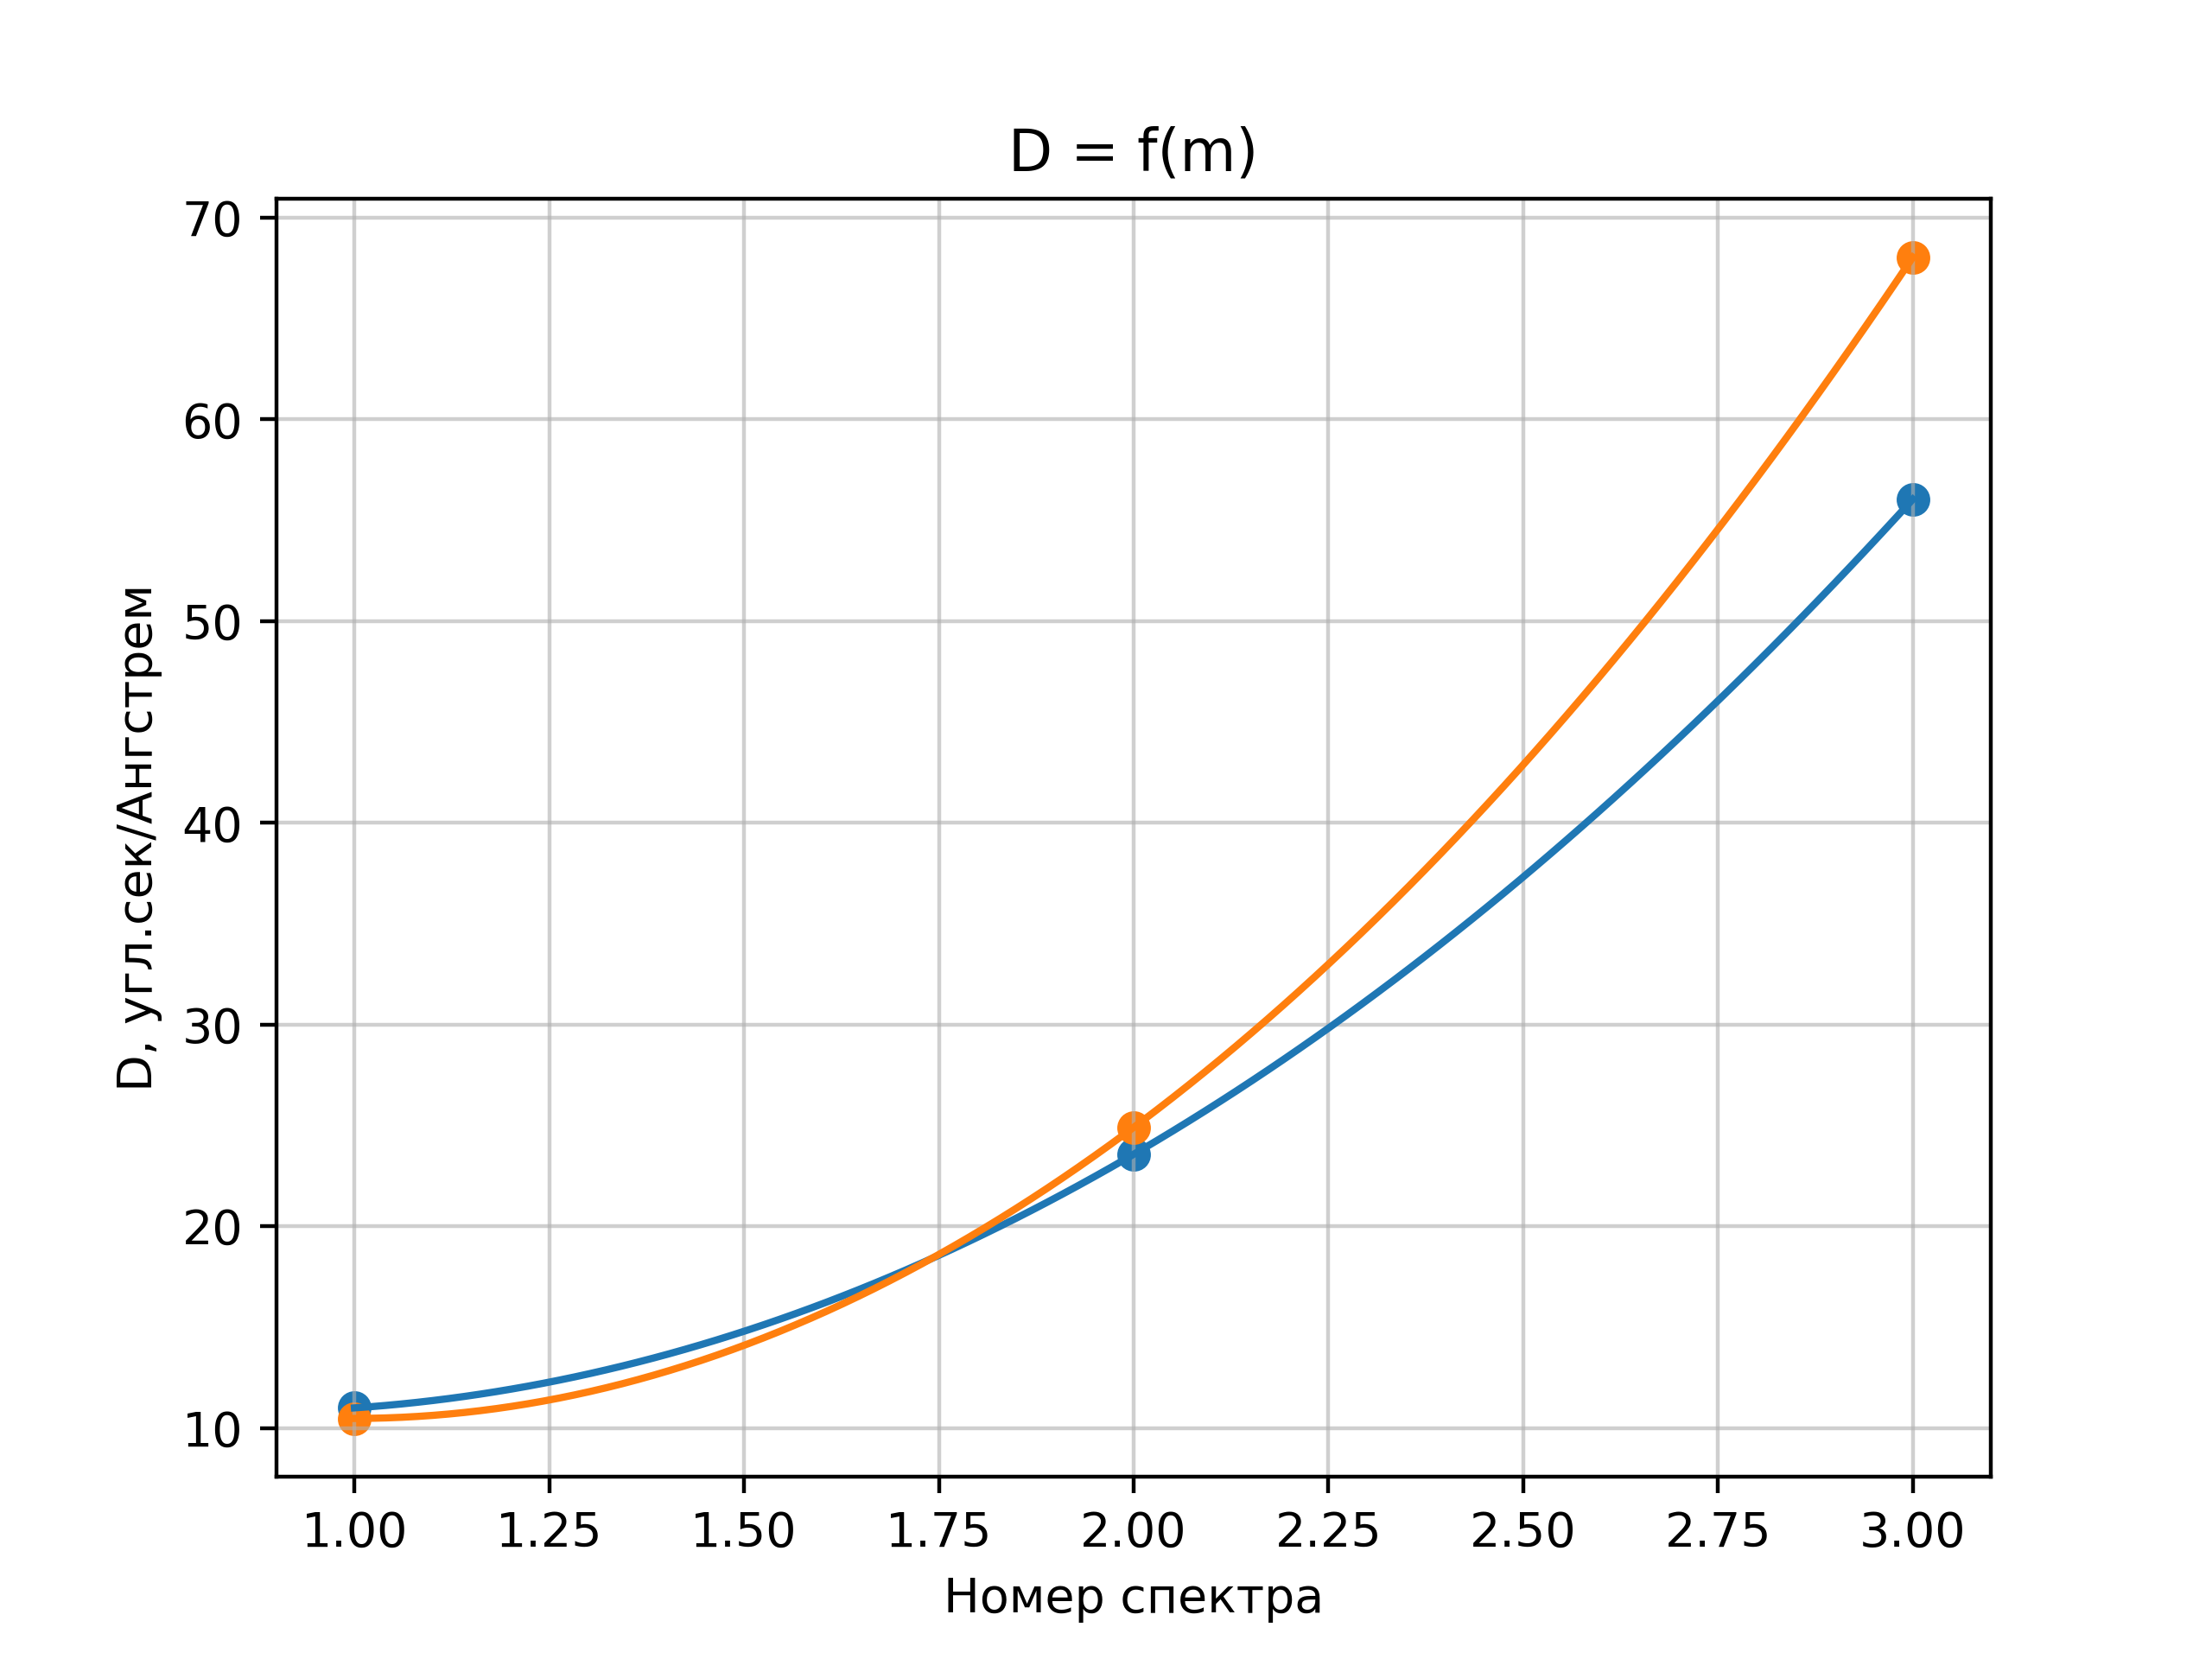
\includegraphics[width=1\textwidth]{plot2.png}
    \caption{Графики для угловых дисперсий}
    \label{fig:plot2}
\end{figure}

Как можно видеть, дисперсия возрастает с увеличение порядка спектра.

Оценим разрешающую способность R и число эффективно работающих штрихов N, а так же эффективный размер l:

\begin{equation*}
	R \approx \frac{\varphi}{\Delta\varphi} \approx \frac{60332}{231} \approx 261
\end{equation*}

\begin{equation*}
	R_{\lambda} \approx \frac{\lambda}{\Delta\lambda} \approx \approx \frac{577}{2,1} \approx 274
\end{equation*}

\begin{equation*}
	N \approx \frac{R}{m} \approx 261
\end{equation*}

\begin{equation*}
	l \approx Nd \approx 0,5 \text{ мм}
\end{equation*}

\section{Выводы}
В работе были исследованы спектральные линии ртути, определен шаг решетки, угловая дисперсия и эффективный размер.
Период решетки d сошелся с реальным в пределах погрешности.
\end{document}